% This is my tamplate for presentations of diploma
% 

\documentclass[ucs]{beamer}
\usepackage{beamerthemeshadow}
\usepackage[T2A]{fontenc}
\usepackage[utf8]{inputenc}
\usepackage[english,ukrainian]{babel}
\usepackage{amssymb,amsfonts,amsmath}
\usepackage{cite,enumerate,float,indentfirst}
% \usepackage[dvips]{graphicx}
\usepackage{graphicx,epstopdf} % epstopdf-convert eps files to pdf
\graphicspath{{fig/},{software/}} % look up folders for figures

\usepackage{wrapfig}

\usepackage{color} 
\usepackage{xcolor} 

\usepackage{helvet} % set font family for whole document
\usefonttheme[onlymath]{serif} % Set font family only for math mode

% \usepackage[warn]{mathtext}
 
% arev, avant, bookman, chancery, charter, euler, helvet, lmodern, mathtime,
% mathptm, mathptmx, newcent, palatino, pifont, utopia.



\begin{document}
\title{Інтегрована інерціально-супутникова система навігації, що базується на принципах комплексної обробки інформації
з використанням калманівської фільтрації}  
% \author{доповідач:Микола Новік\\ керівник: Мар’ясова Т.І.}
\author{Микола Новік}
\date{\today} 

% First Slide, title page
\begin{frame}
\titlepage
\end{frame}

% Just print table of contents
\begin{frame}\frametitle{Зміст доповіді}
\tiny
\tableofcontents
\end{frame} 

%intro
\section{Постановка задачі та вибір системи} 
\subsection{Постановка задачі та вибір системи} 
\begin{frame}\frametitle{Постановка задачі комплексування}
\small
\beamerbutton{\smallПостановка задачі}: дослідження можливостей комплексування навігаційної інформації двох систем, що є на борту сучасного літака: безплатформенної інерціальної навігаційної системи і супутникової високоточної навігаційної системи.\\
\centering \line(1,0){200}

\begin{block}<+->{В результатi комплексування IНС та СНС досягаються:}
\tiny
\begin{enumerate}
\item  пiдвищення точностi визначення координат, висоти, швидкостi i часу споживача;
\item  уточнення кутiв орiєнтацiї (курсу, крену i тангажа);
\item  оцiнка й уточнення параметрiв калiбрування навiгацiйних датчикiв,
таких, як дрейфи гiроскопiв, масштабнi коефiцiєнти, зсуви акселерометрiв тощо;
\item  забезпечення на цiй основi безперервностi навiгацiйних визначень на всiх етапах руху, у тому числi i при тимчасовiй непрацездатностi приймача СНС у випадках впливу завад або енергiйних маневрiв ЛА.

\end{enumerate}
\end{block}

\end{frame} 

%%%%<<<<<<<<<<<<<<<<<<<<<<<<<<<<<<<<<<<<<<<<<<<<<<<<<<<<<<<<<<<<<<<<<<<<<<<<<<<<<<<
\subsection{Вибір варіанту комплексування ІСНС } 
\begin{frame}\frametitle{Варіанти інтегрування ІСНС} 

\tiny
\begin{block}{Роздільна}
Надмірність, обмеженість похибок оцінок місця розташування і швидкості, 
наявність інформації про орієнтацію і кутову швидкість, висока швидкість видачі інформації, 
мінімальні зміни в бортовій апаратурі
\end{block}

\begin{exampleblock}{Слабко зв'язана}
Усі перераховані особливості роздільних систем, плюс більш 
швидке відновлення слідкування за кодом і фазою сигналів СНС, виставлення та калібрування 
БІНС у польоті, як наслідок -- підвищена точність під час відсутності сигналу СНС
\end{exampleblock}


\begin{block}{Жорстко зв'язана}
Подальше поліпшення точності і калібрування, підвищена стійкість слідкування 
за сигналами СНС при маневрах ЛА, підвищена завадостійкість 
\end{block}

\begin{block}{Глибоко інтегрована}
Єдиний фільтр усуває проблему ``каскадного'' включення 
фільтрів, компактність, знижені вимоги з енергозабезпечення. Недоліки: вектор стану 
містить до 40 компонентів, тому фільтр складно реалізувати; необхідність розробки 
спеціальних датчиків 
\end{block}
\end{frame}
%%%%<<<<<<<<<<<<<<<<<<<<<<<<<<<<<<<<<<<<<<<<<<<<<<<<<<<<<<<<<<<<<<<<<<<<<<<<<<<<<<<


\subsection{Схема комплексування ІСНС }
\begin{frame} \frametitle{Схема ІСНС} 
\begin{figure}[here]
\centering
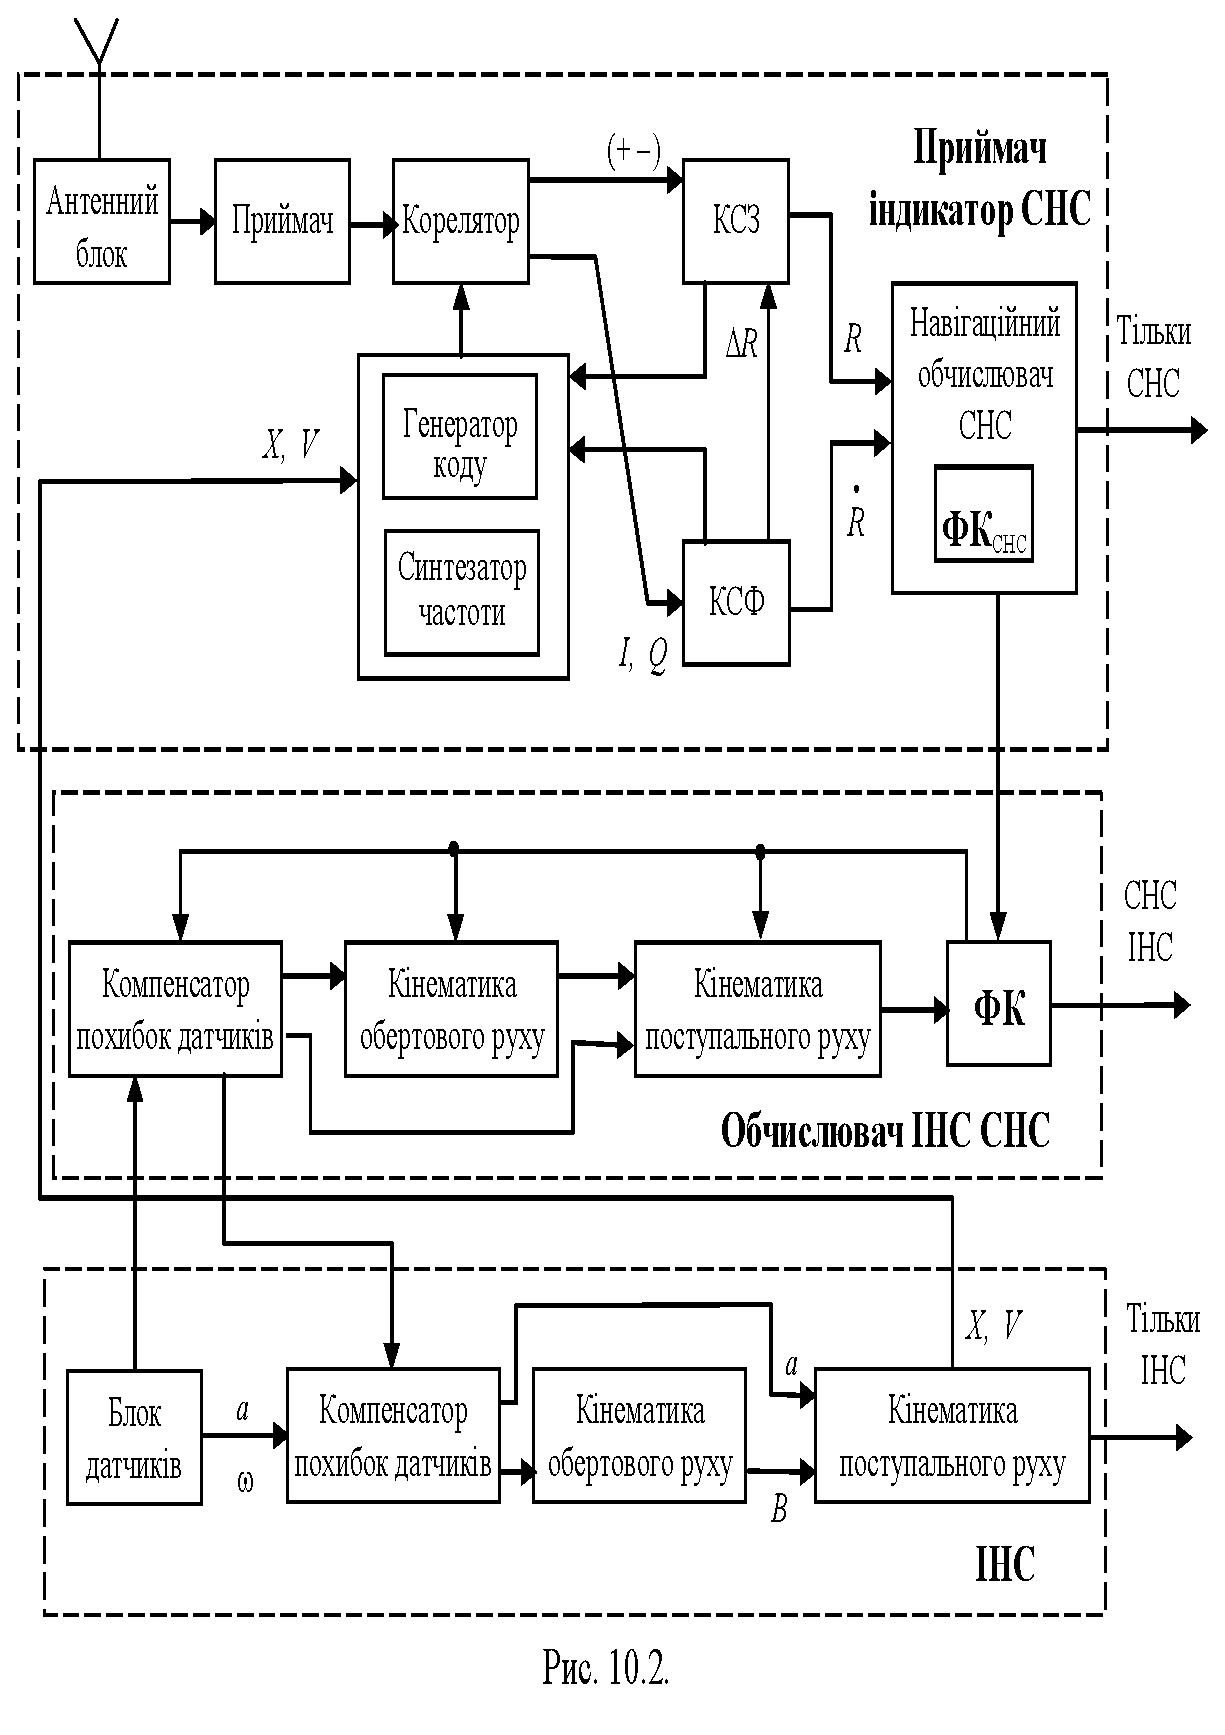
\includegraphics[width=90mm,height=65mm]{isns_loosly}
\caption{Слабко зв’язана схема}
%\label{fig:isns_loosly}
\end{figure}
\end{frame}
%%%%<<<<<<<<<<<<<<<<<<<<<<<<<<<<<<<<<<<<<<<<<<<<<<<<<<<<<<<<<<<<<<<<<<<<<<<<<<<<<<<

\section{Модель системи }
\subsection{Система в просторі станів}
\begin{frame}[shrink=5] \frametitle{Система в просторі станів} 



\begin{columns}[t]
\begin{column}{5cm}
\noindent 
Вектор стану системи
\begin{equation*}
\tiny
% \bar{X}= 
\left[ \begin{array}{l}
{\Delta R_{E}}\\
{\Delta R_{N}}\\
{\Delta h}\\
{\Delta V_{E}}\\
{\Delta V_{N}}\\
{\Delta V_{h}}\\
{\alpha_{E}}\\
{\alpha_{N}}\\
{\alpha_{h}}\\
{\varepsilon_{c1}}\\
{\varepsilon_{c2}}\\
{\varepsilon_{c3}}\\
{\Delta a_{c1}} \\
{ \Delta a_{c2}}\\
{\Delta a_{c3}}\\
{\Delta h_{\text{БВ}}}\\
{\Delta R_{Ec}}\\
{\Delta R_{Nc}}\\
{\Delta h_{c}}\\
{\Delta V_{Ec}}\\
{\Delta V_{Nc}}\\
{\Delta V_{hc}}
\end{array} \right]=
\left[\begin{array}{l}
{\text{Пом. координ. E}}\\
{\text{Пом. координ. N}}\\
{\text{Пом. по висоті}}\\
{\text{Пом. по швидкості E}}\\
{\text{Пом. по швидкості N}}\\
{\text{Пом. по швидкості H}}\\
{\text{Пом. тригранника E}}\\
{\text{Пом. тригранника N}}\\
{\text{Пом. тригранника H}}\\
{\text{Дрейф гіроскопа E}}\\
{\text{Дрейф гіроскопа N}}\\
{\text{Дрейф гіроскопа H}}\\
{\text{Дрейф акселерометра E}} \\
{\text{Дрейф акселерометра N}}\\
{\text{Дрейф акселерометра H}}\\
{\text{Пом. баровисотоміра}}\\
{\text{Кор. пом. коорд. СНС E}}\\
{\text{Кор. пом. коорд. СНС N}}\\
{\text{Кор. пом. коорд. СНС H}}\\
{\text{Кор. пом. швид. СНС E}}\\
{\text{Кор. пом. швид. СНС N}}\\
{\text{Кор. пом. швид. СНС H}}\\
\end{array} \right]  
\end{equation*}

\end{column}
\begin{column}{5cm}
Моедель системи в просторі станів.\\

\tiny

$\bar{X}_{p,k+1} =\Phi_{p,k} \bar{X}_{p,k} +G_{p,k} \bar{\xi }_{k}$ \\
Матриця динаміки системи\\
$ F_{p,k} =\left(\begin{array}{ccc} 
{F_{k} } & {.} & {.} \\
{.} & {F_{bv}} & {.} \\
{.} & {.} & {F_{sns}} \\
\end{array}\right);$
Коваріаційна матриця шумів\\
$Q_{p,k} =\left(\begin{array}{ccc} 
{Q_{k} } & {.} & {.} \\ 
{.} & {\sigma_{\text{БВ}} \sqrt{\Delta t}} & {.} \\ 
{.} & {.} & {G_{s,k} } \end{array}\right);$
Вимірювання\\
$\bar{Y}_{k} = 
\left(\begin{array}{l}
{\tilde{h}_{k} -\tilde{h}_{\text{БВ},k},}\\
{\tilde{R}_{E,K} -\tilde{R}_{ES,k},}\\
{\tilde{R}_{N,K} -\tilde{R}_{NS,k},}\\
{\tilde{h}_{k} -\tilde{h}_{s,k},}\\
{\tilde{V}_{E,k} -\tilde{V}_{ES,k},}\\
{\tilde{V}_{N,k} -\tilde{V}_{NS,k},}\\
{\tilde{V}_{h,k} -\tilde{V}_{hS,k},}\\
{\tilde{h}_{\text{БВ}} -\tilde{h}_{s,k}}
\end{array} \right) $

\end{column}
\end{columns}


\end{frame}
%%%%<<<<<<<<<<<<<<<<<<<<<<<<<<<<<<<<<<<<<<<<<<<<<<<<<<<<<<<<<<<<<<<<<<<<<<<<<<<<<<<

\subsection{Еволюція стаціонарно закріпленої БІНС} 
\begin{frame}[plain]
\frametitle{Помилка координати}

\begin{figure}[l]
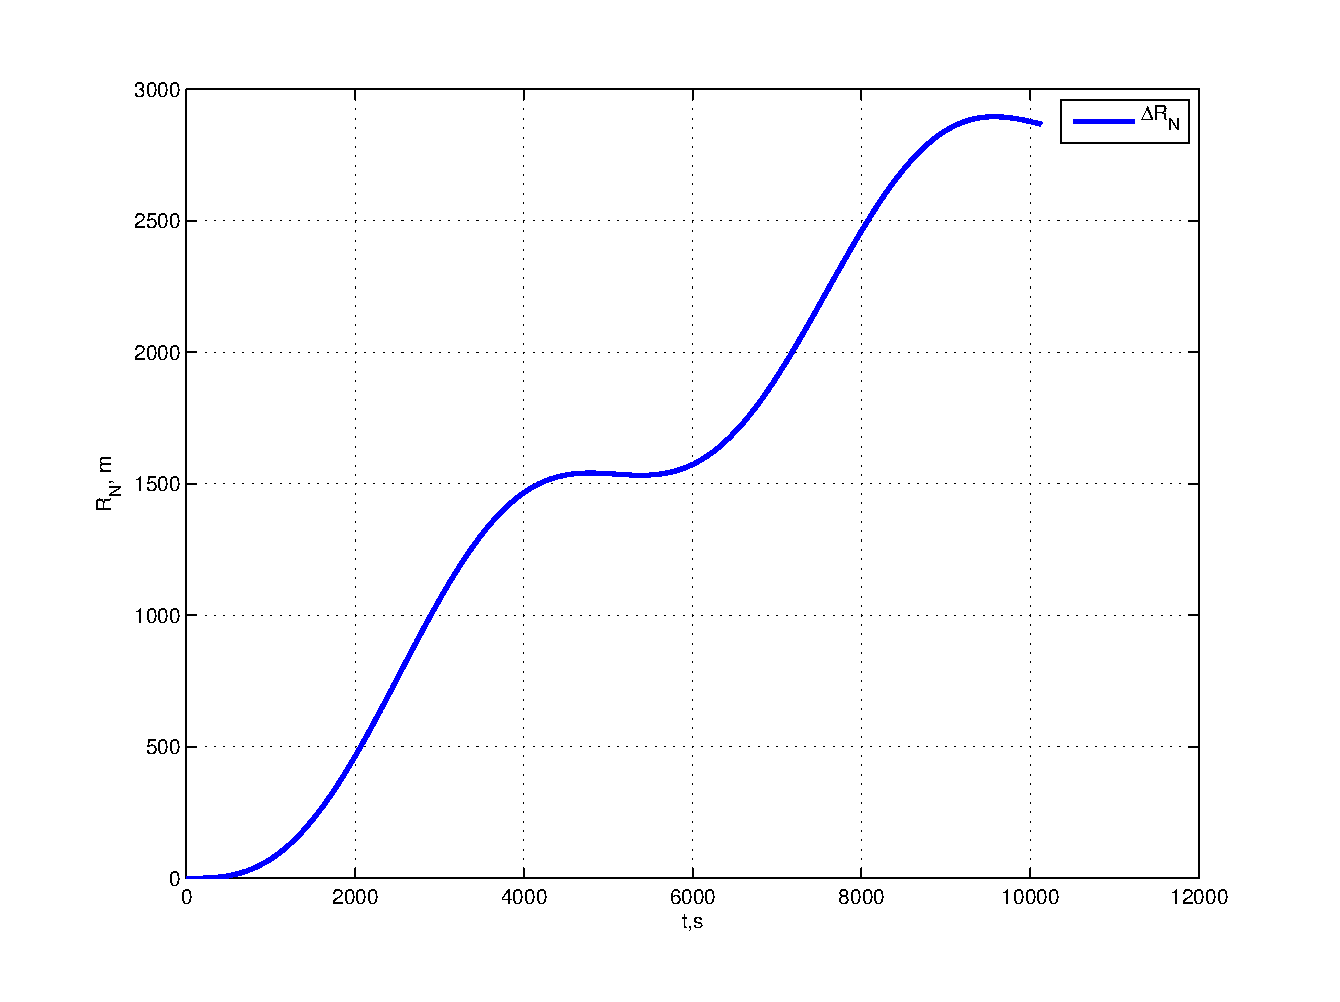
\includegraphics[scale=0.24]{ins_stat_gyro}
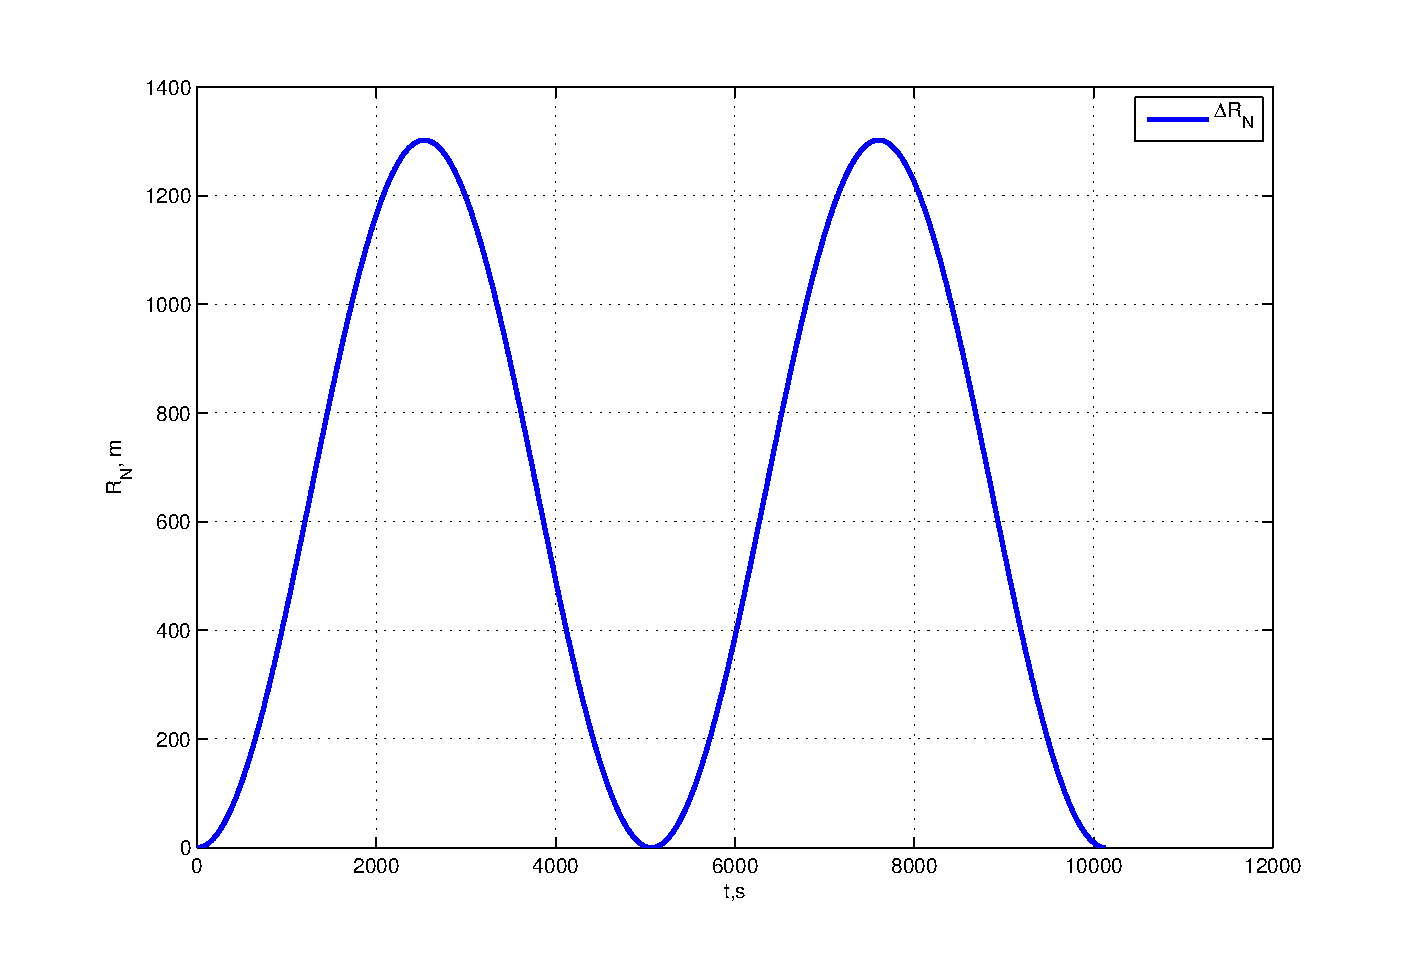
\includegraphics[scale=0.25]{ins_stat_tilt}
\caption{\tiny Еволюція похибки за умови, дрейфу гіроскопа $0.01 deg/h$; Еволюція похибки за умови, похибки координатного тригранника $10^{-3} rad$}
\label{fig:sdins2}
\end{figure}
\end{frame}

%%%%<<<<<<<<<<<<<<<<<<<<<<<<<<<<<<<<<<<<<<<<<<<<<<<<<<<<<<<<<<<<<<<<<<<<<<<<<<<<<<<
\subsection{Сумарна похибка БІНС} 
\begin{frame}[plain]
\frametitle{Сумарна похибка БІНС}

\begin{figure}[l]
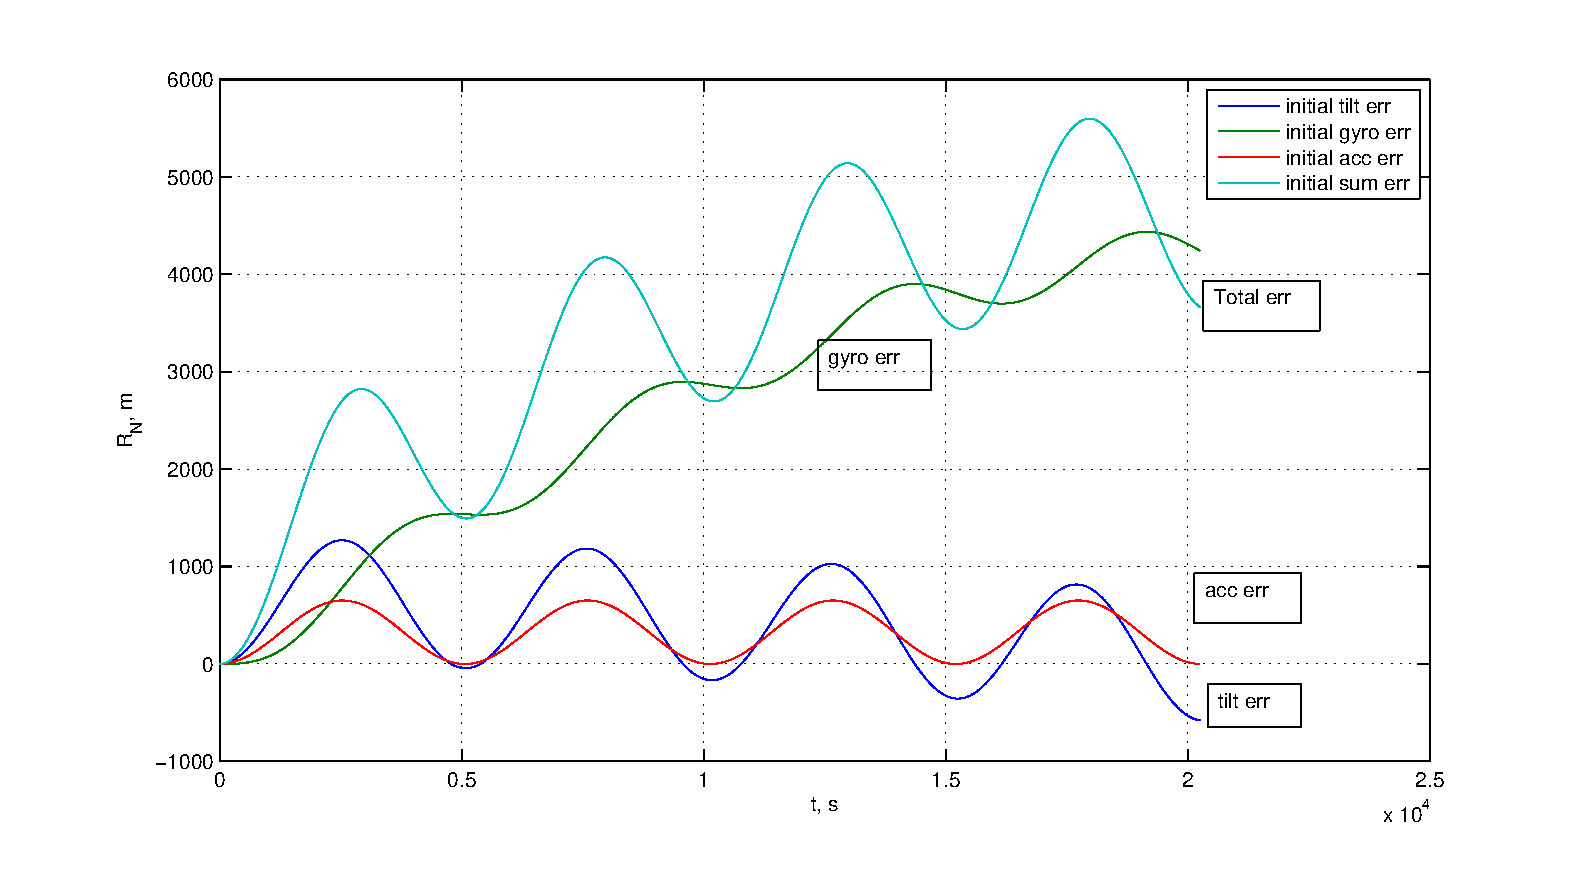
\includegraphics[scale=0.45]{ins_stat_sum}

\caption{\tinyЕволюція сумарної похибки по координаті за умови,
дрейфу гіроскопа   $0.01 deg/h$,похибки координатного тригранника $10^{-3} rad$, та зміщенням акселерометра $10^{-4} m/s^2$}
\label{fig:sdins2}
\end{figure}
\end{frame}
%%%%<<<<<<<<<<<<<<<<<<<<<<<<<<<<<<<<<<<<<<<<<<<<<<<<<<<<<<<<<<<<<<<<<<<<<<<<<<<<<<<
\subsection{Навігаційний фільтр} 
\begin{frame}[plain]
\frametitle{Навігаційний фільтр}
\begin{figure}[l]
\includegraphics[scale=0.15]{kalman_diag}
% \caption{\tinyЕволюція сумарної }
\end{figure}
\begin{block}{Фільтр Калмана}
\small
Прогноз: \\
$\begin{array}{l} 
{\hat{\bar{X}}_{p,k}(-) =\Phi_{p,k-1} \hat{\bar{X}}_{p,k-1}(+) ,} \\ 
{P_{k}(-) =\Phi_{p,k-1} P_{k-1}(+) \Phi ^{T}_{p,k-1} +G_{p,k-1} G_{p,k-1}^{T} ;} \end{array} $ \\
Корекція:\\
$\begin{array}{l} 
{\hat{\bar{X}}_{p,k}(+)=\hat{\bar{X}}_{p,k}(-) + K_{k} (\bar{Y}_{k} -H\hat{\bar{X}}_{p,k} )} \\ 
{P_{k}(+)={\color{blue}(E-K_{k} H)P_{k}(-) \left(E-K_{k} H\right)^{T}} +{\color{red} K_{k} Q_{p,k} Q_{p,k} ^{T} K_{k}^{T}} } 
\end{array} $ \\
Коефіцієнт Калмана:\\
$K_{k} =P_{k}(-) H^{T} (HP_{k}(-) H^{T} +Q_{p,k} Q_{p,k} ^{T} )^{-1} $
\end{block}
\end{frame}
%%%%<<<<<<<<<<<<<<<<<<<<<<<<<<<<<<<<<<<<<<<<<<<<<<<<<<<<<<<<<<<<<<<<<<<<<<<<<<<<<<<
\subsection{Траєкторія руху ЛА} 
\begin{frame}%[plain]
\frametitle{Траєкторія руху ЛА та кути крену, курса і тангажа}
\noindent
\begin{figure}[l]
\noindent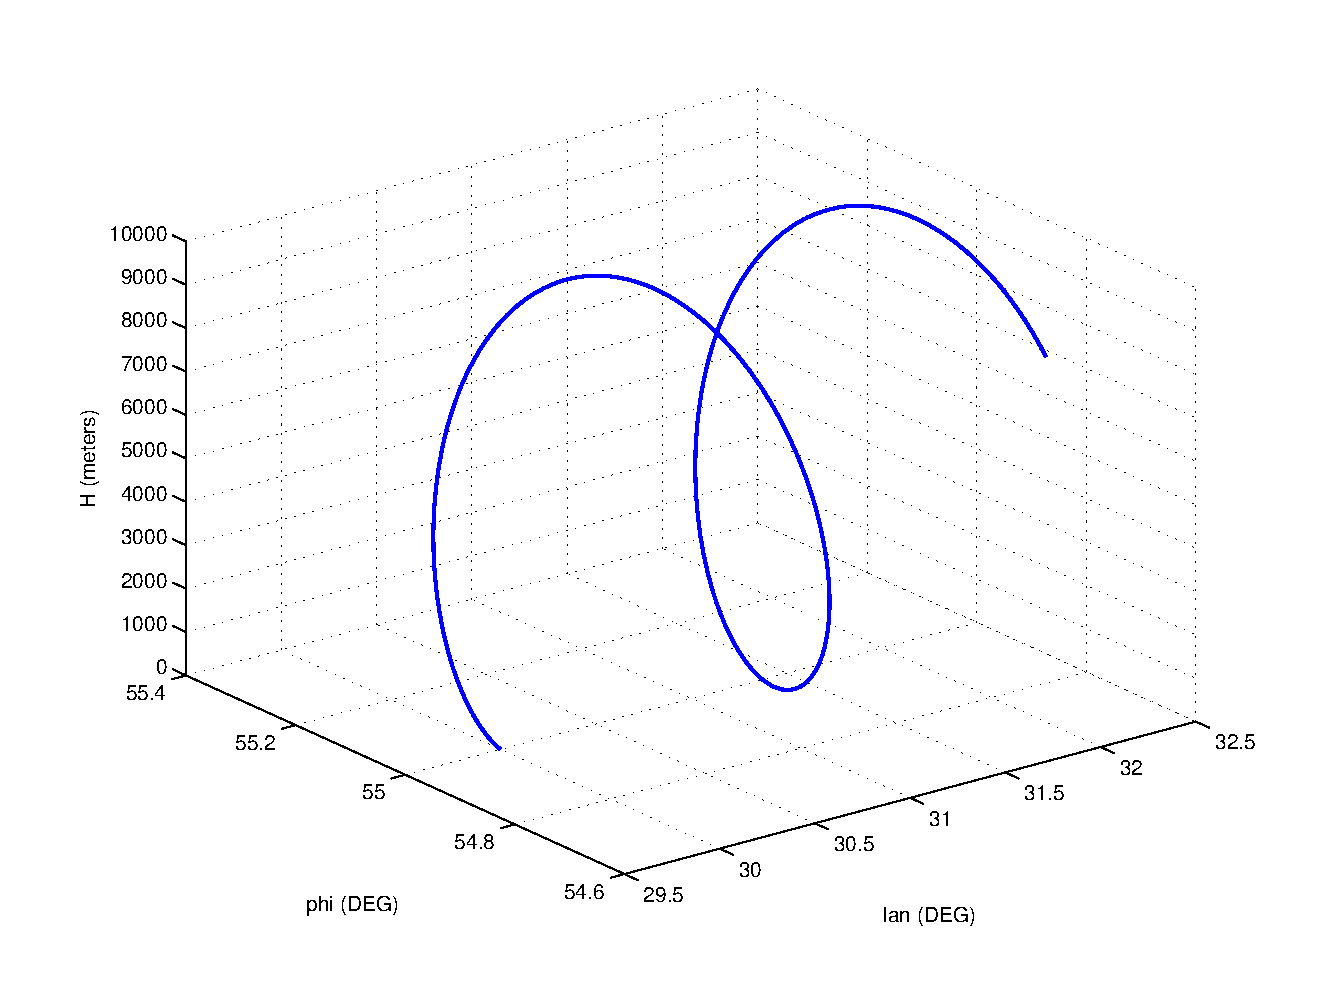
\includegraphics[scale=0.28]{path_3d}
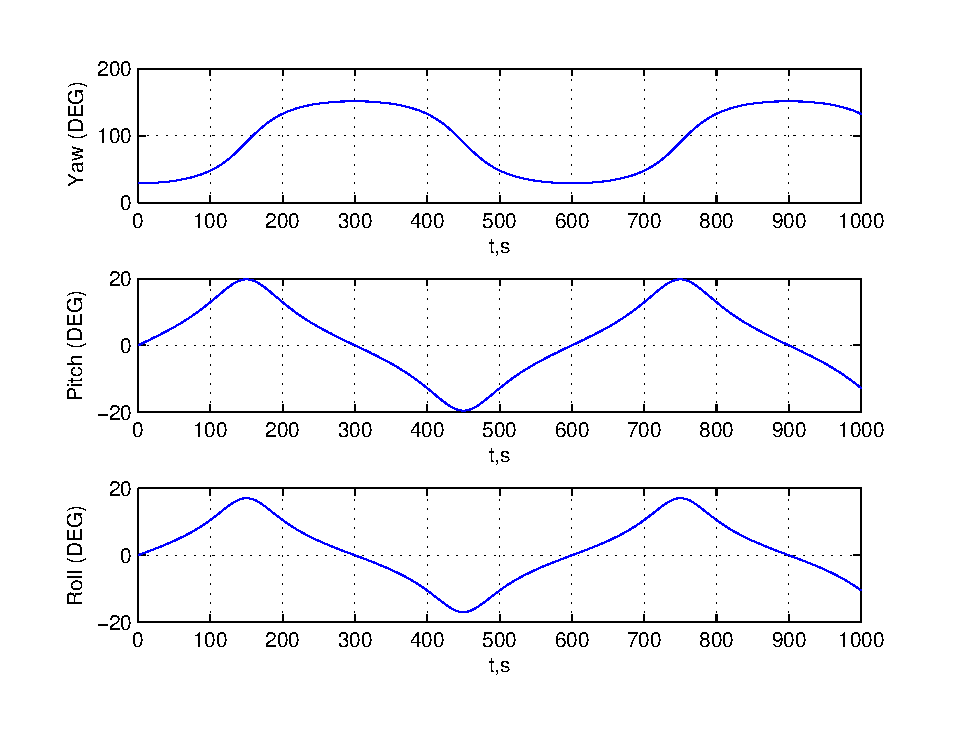
\includegraphics[scale=0.35]{path_PYR}
\caption{\tiny Траєкторія руху ЛА та його кути орієнтації }
\end{figure}
\end{frame}
%%%%<<<<<<<<<<<<<<<<<<<<<<<<<<<<<<<<<<<<<<<<<<<<<<<<<<<<<<<<<<<<<<<<<<<<<<<<<<<<<<<
\section{Результати моделювання ІСНС} 
\subsection{Поихибка оцінки по координаті} 
\begin{frame}%[plain]
\frametitle{Поихибка оцінки по координаті}
\noindent
\begin{figure}
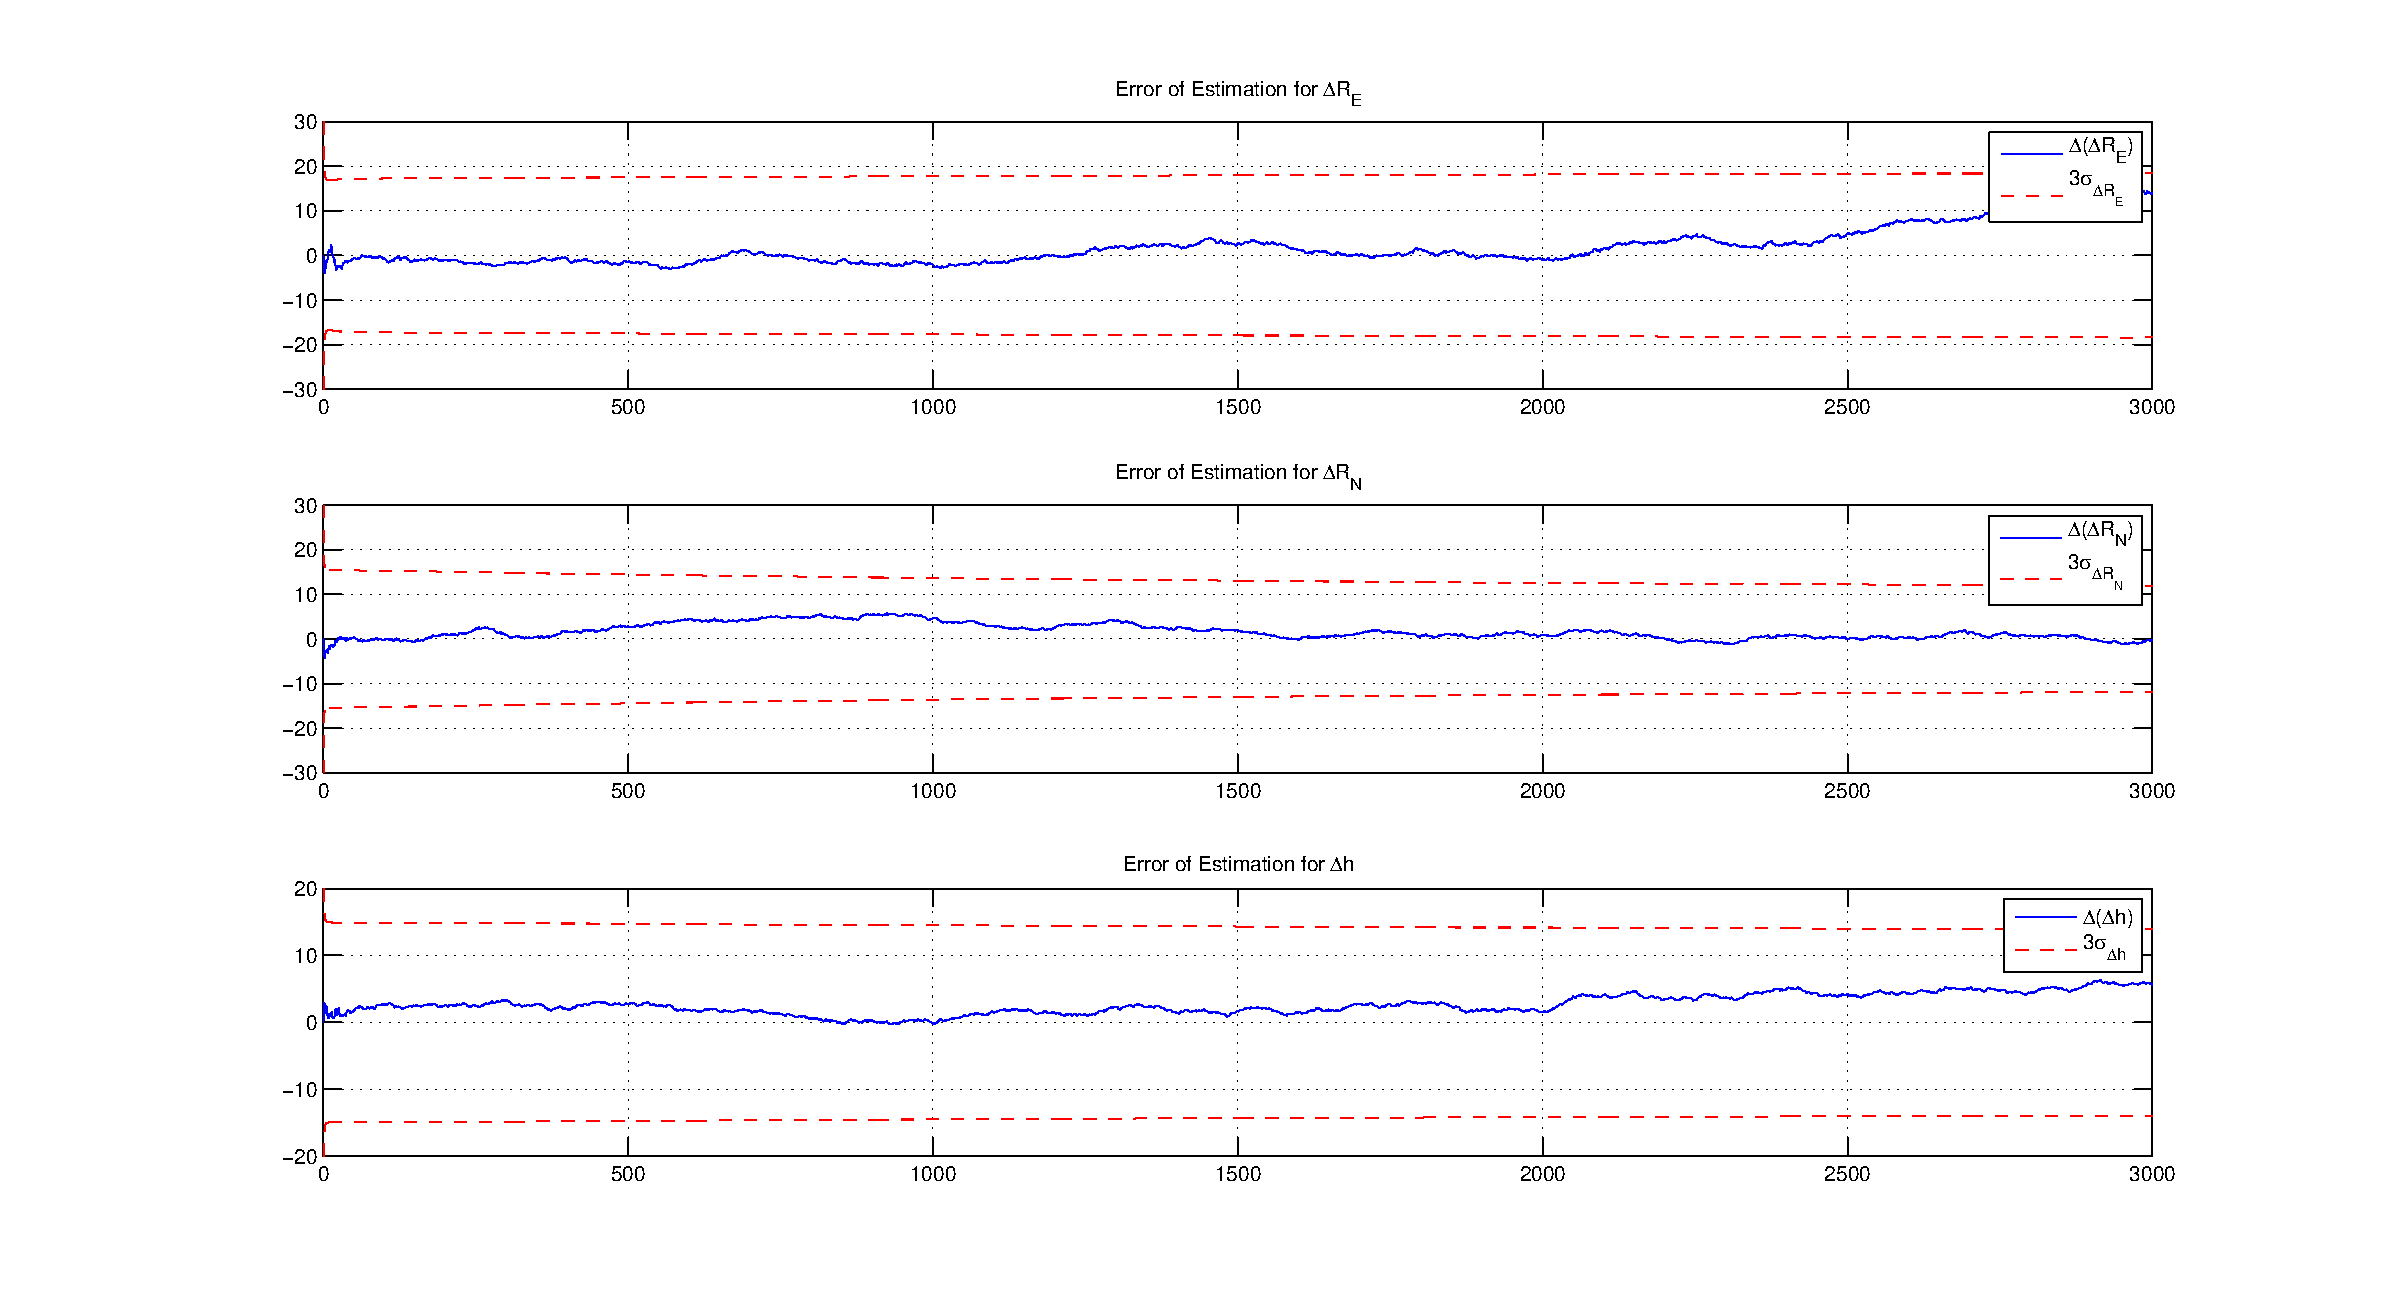
\includegraphics[scale=0.3]{ErrEstCovR}
% \caption{\tiny Траєкторія руху ЛА та його кути орієнтації }
\end{figure}
\end{frame}
%%%%<<<<<<<<<<<<<<<<<<<<<<<<<<<<<<<<<<<<<<<<<<<<<<<<<<<<<<<<<<<<<<<<<<<<<<<<<<<<<<<
\subsection{Поихибка оцінки по швидкості} 
\begin{frame}%[plain]
\frametitle{Поихибка оцінки по швидкості}
\noindent
\begin{figure}
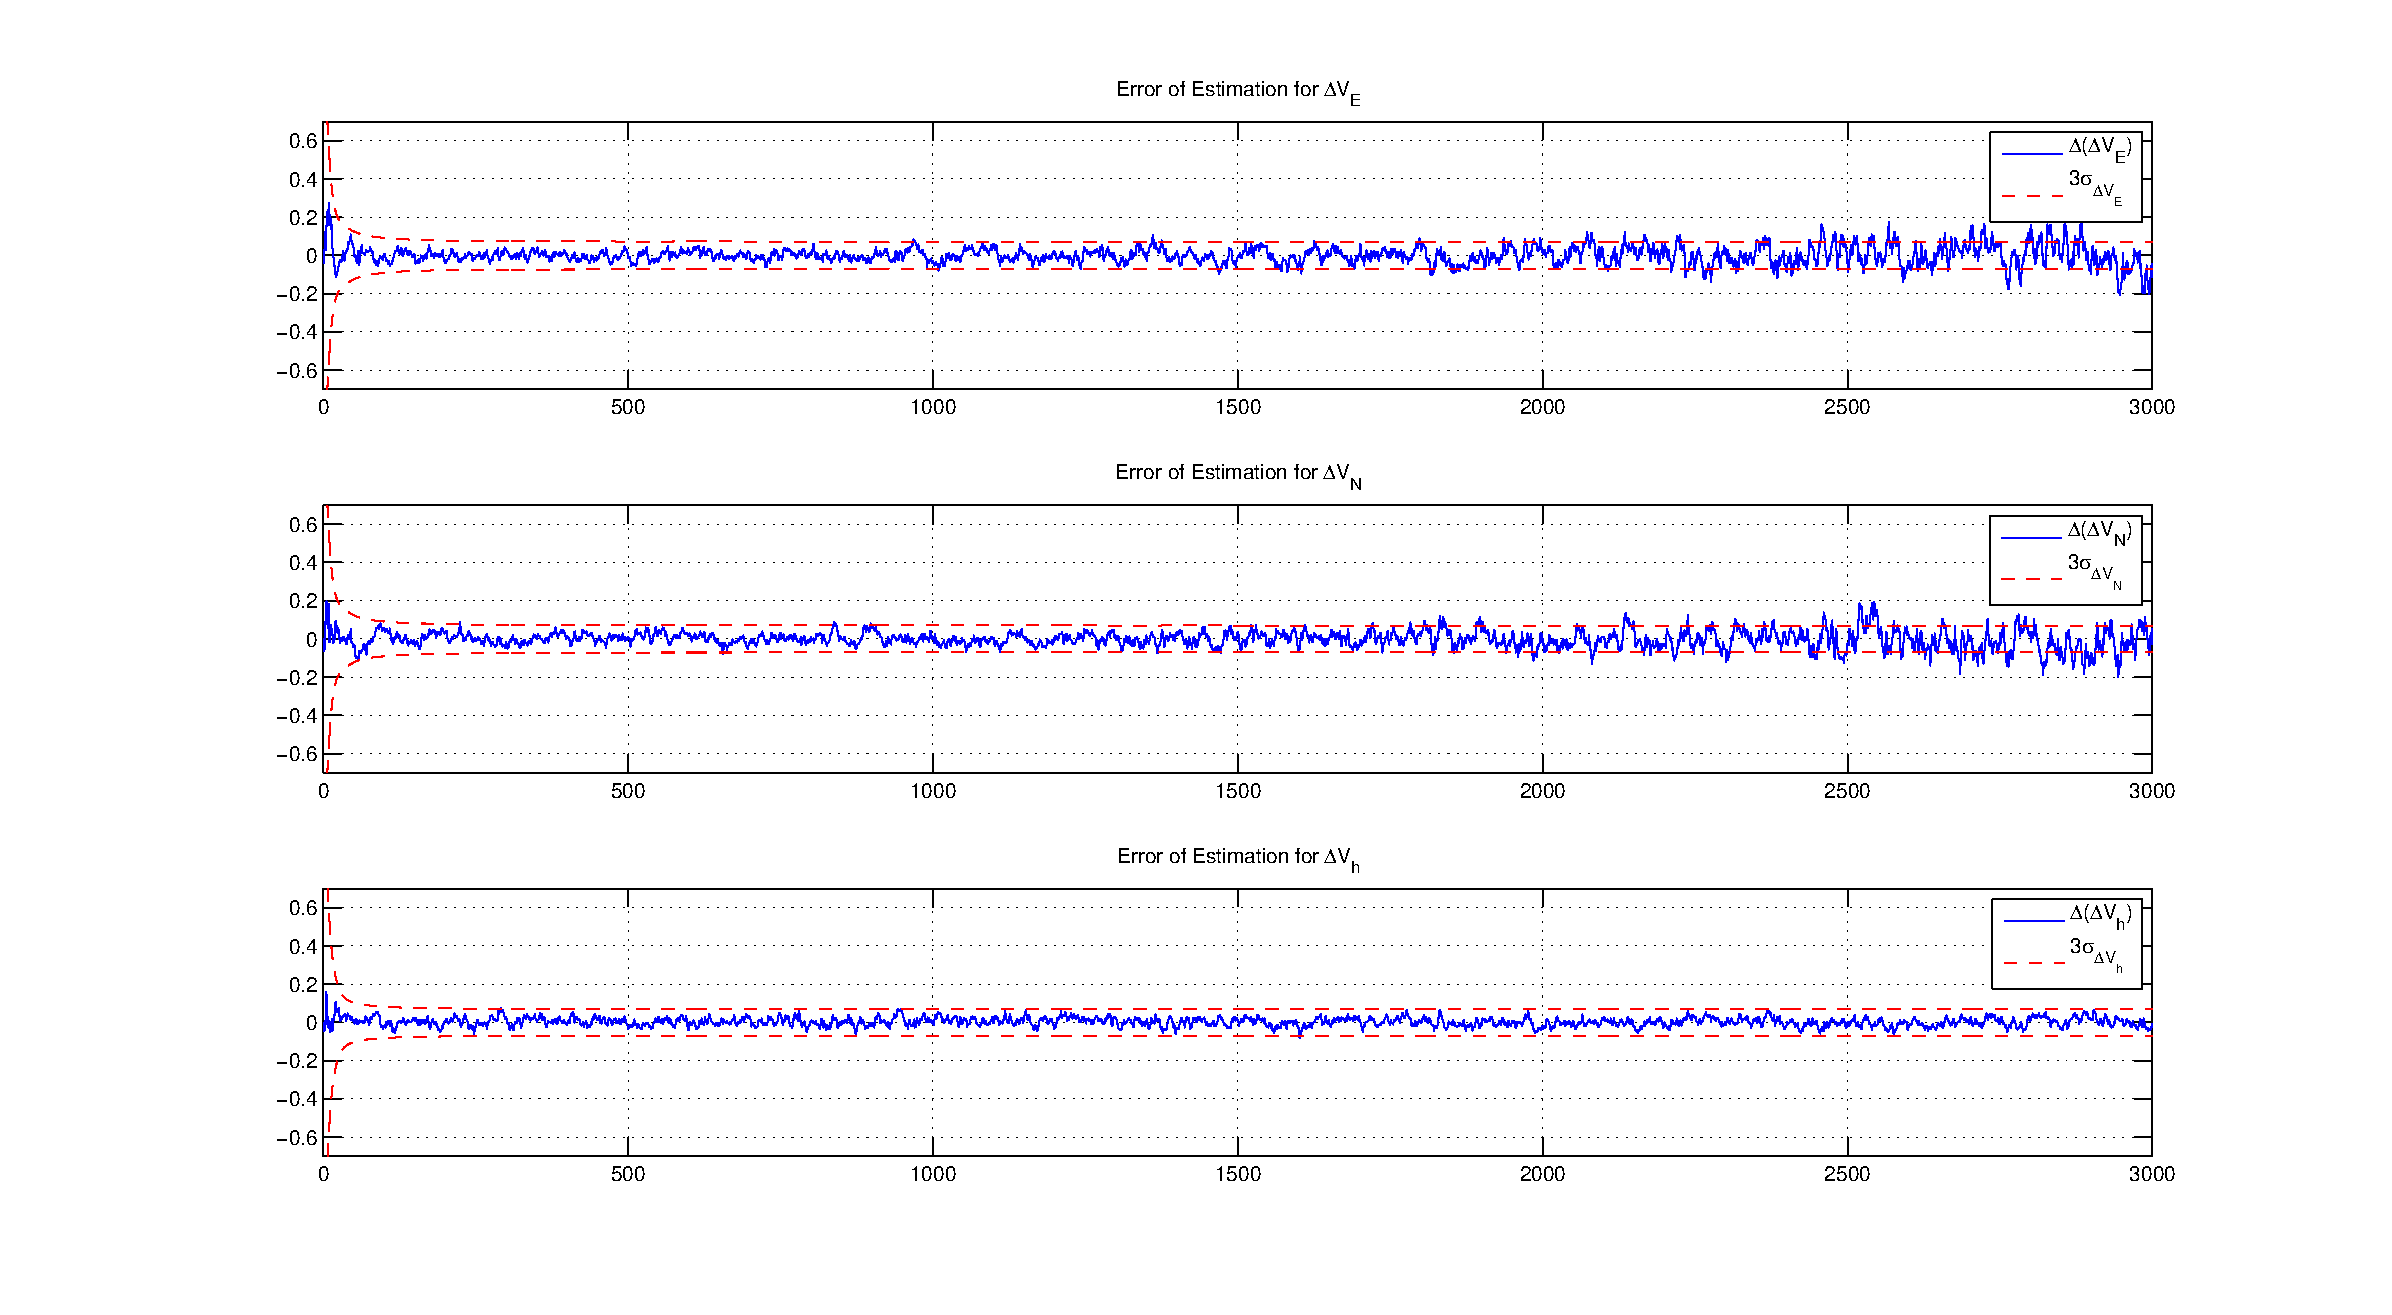
\includegraphics[scale=0.3]{ErrEstCovV}
% \caption{\tiny Траєкторія руху ЛА та його кути орієнтації }
\end{figure}
\end{frame}

%%%%<<<<<<<<<<<<<<<<<<<<<<<<<<<<<<<<<<<<<<<<<<<<<<<<<<<<<<<<<<<<<<<<<<<<<<<<<<<<<<<
\subsection{Поихибка оцінки по орієнтації} 
\begin{frame}%[plain]
\frametitle{Поихибка оцінки по орієнтації}
\noindent
\begin{figure}
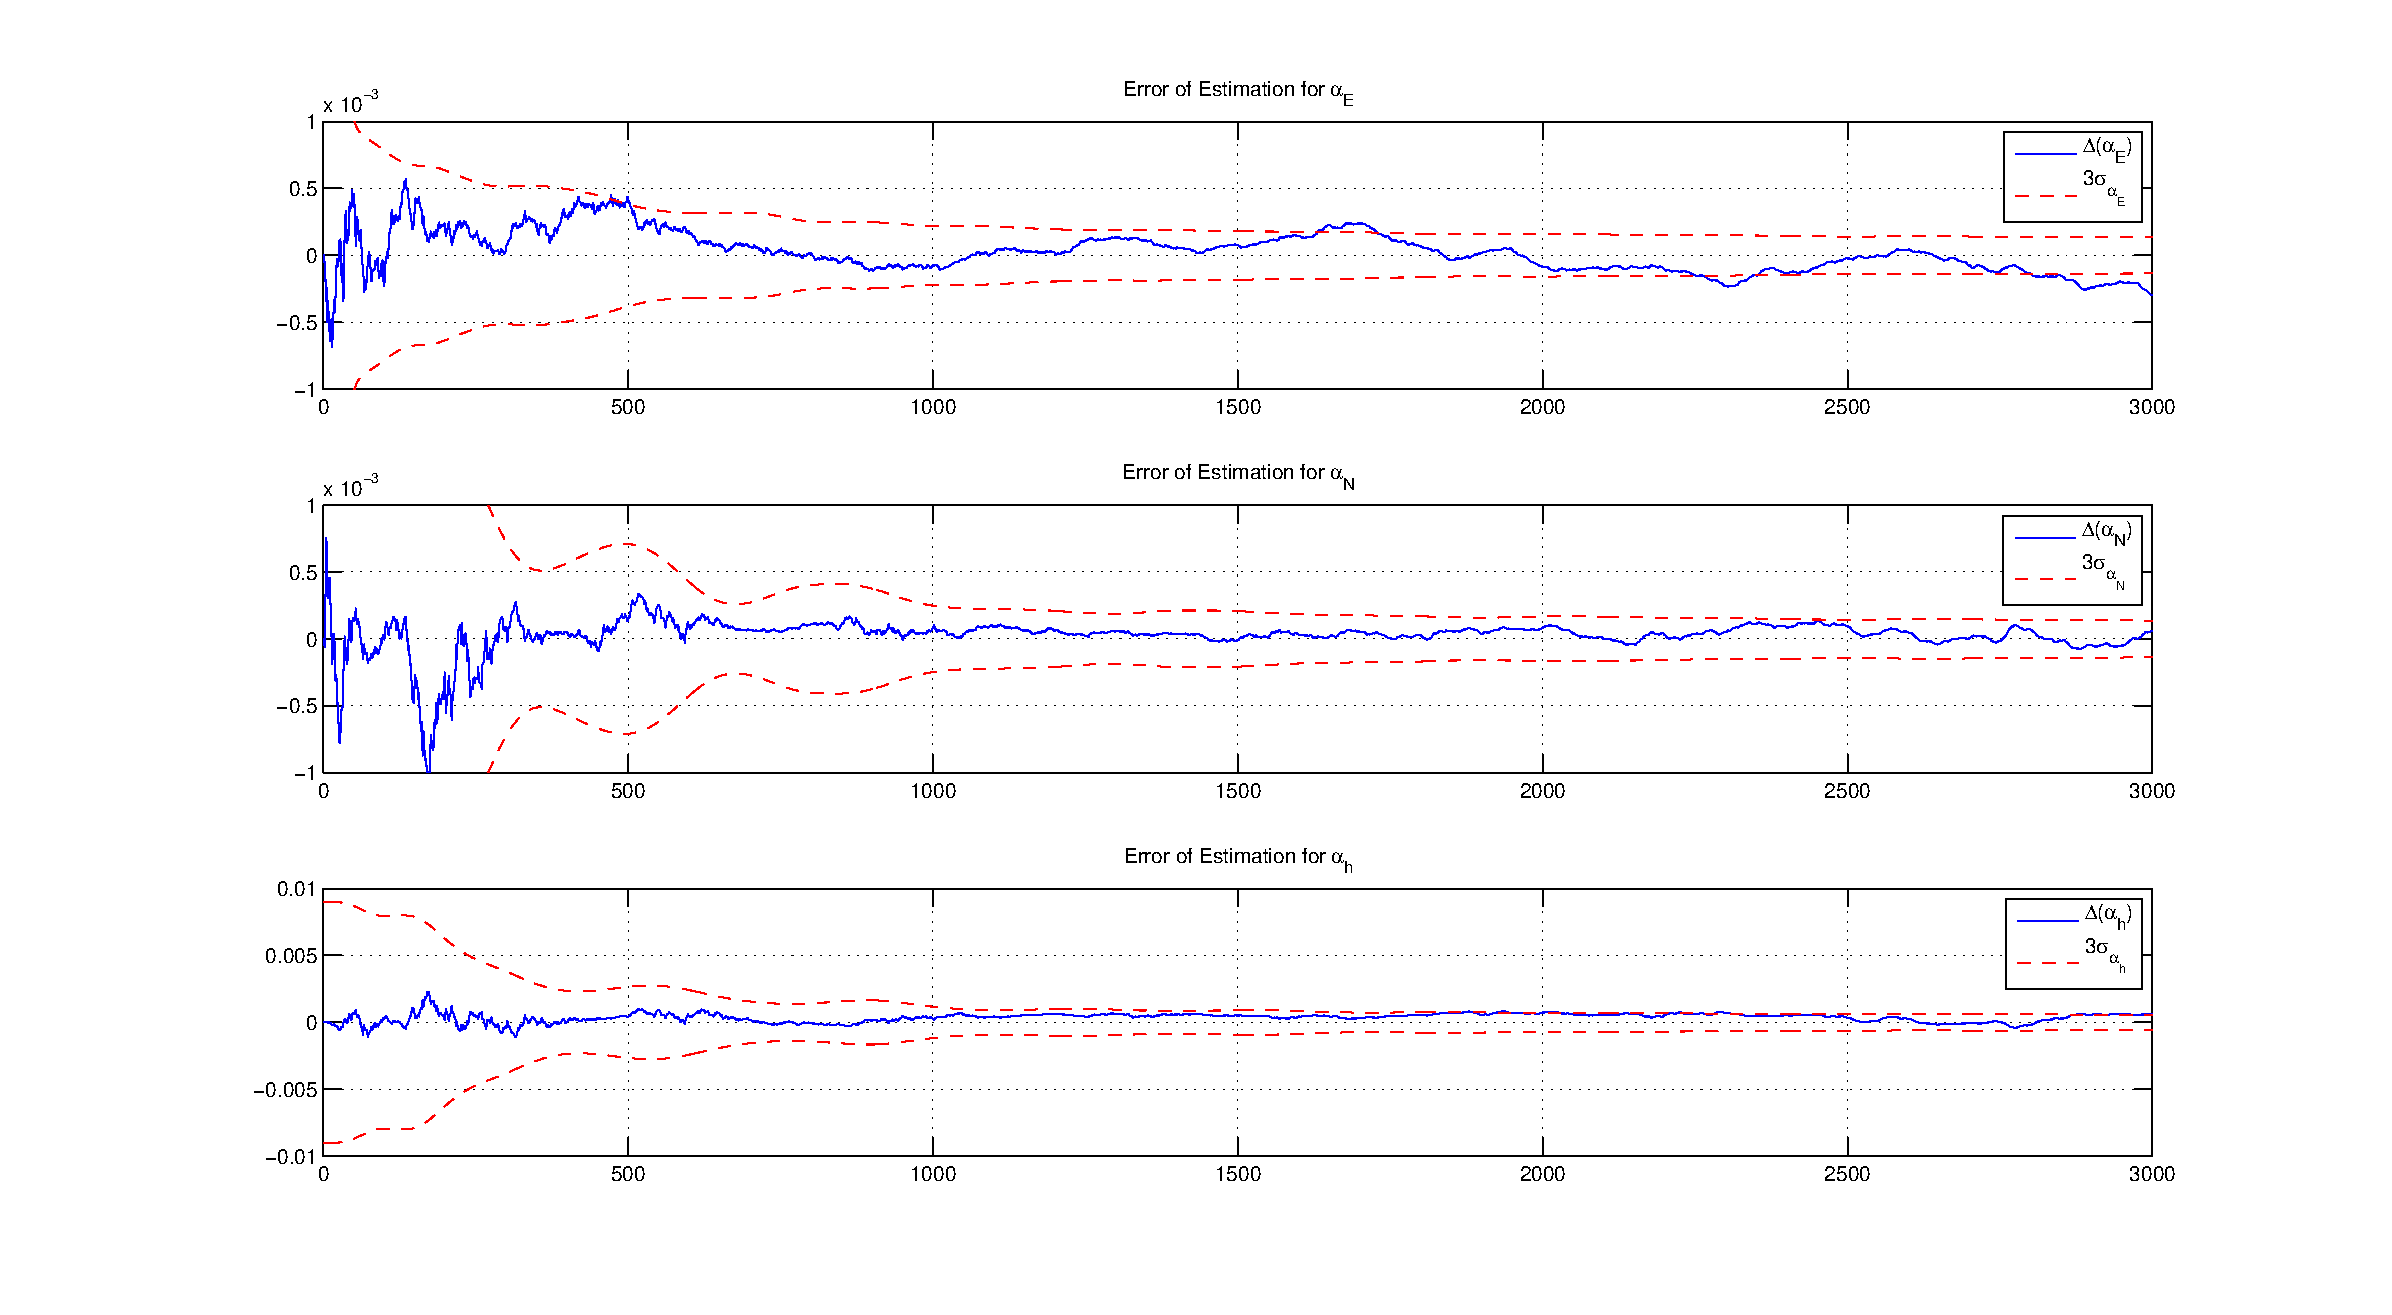
\includegraphics[scale=0.3]{ErrEstCovAlph}
% \caption{\tiny Траєкторія руху ЛА та його кути орієнтації }
\end{figure}
\end{frame}
%%%%<<<<<<<<<<<<<<<<<<<<<<<<<<<<<<<<<<<<<<<<<<<<<<<<<<<<<<<<<<<<<<<<<<<<<<<<<<<<<<<
\subsection{Поихибка оцінки дрейфів гіроскопів} 
\begin{frame}%[plain]
\frametitle{Поихибка оцінки дрейфів гіроскопів}
\noindent
\begin{figure}
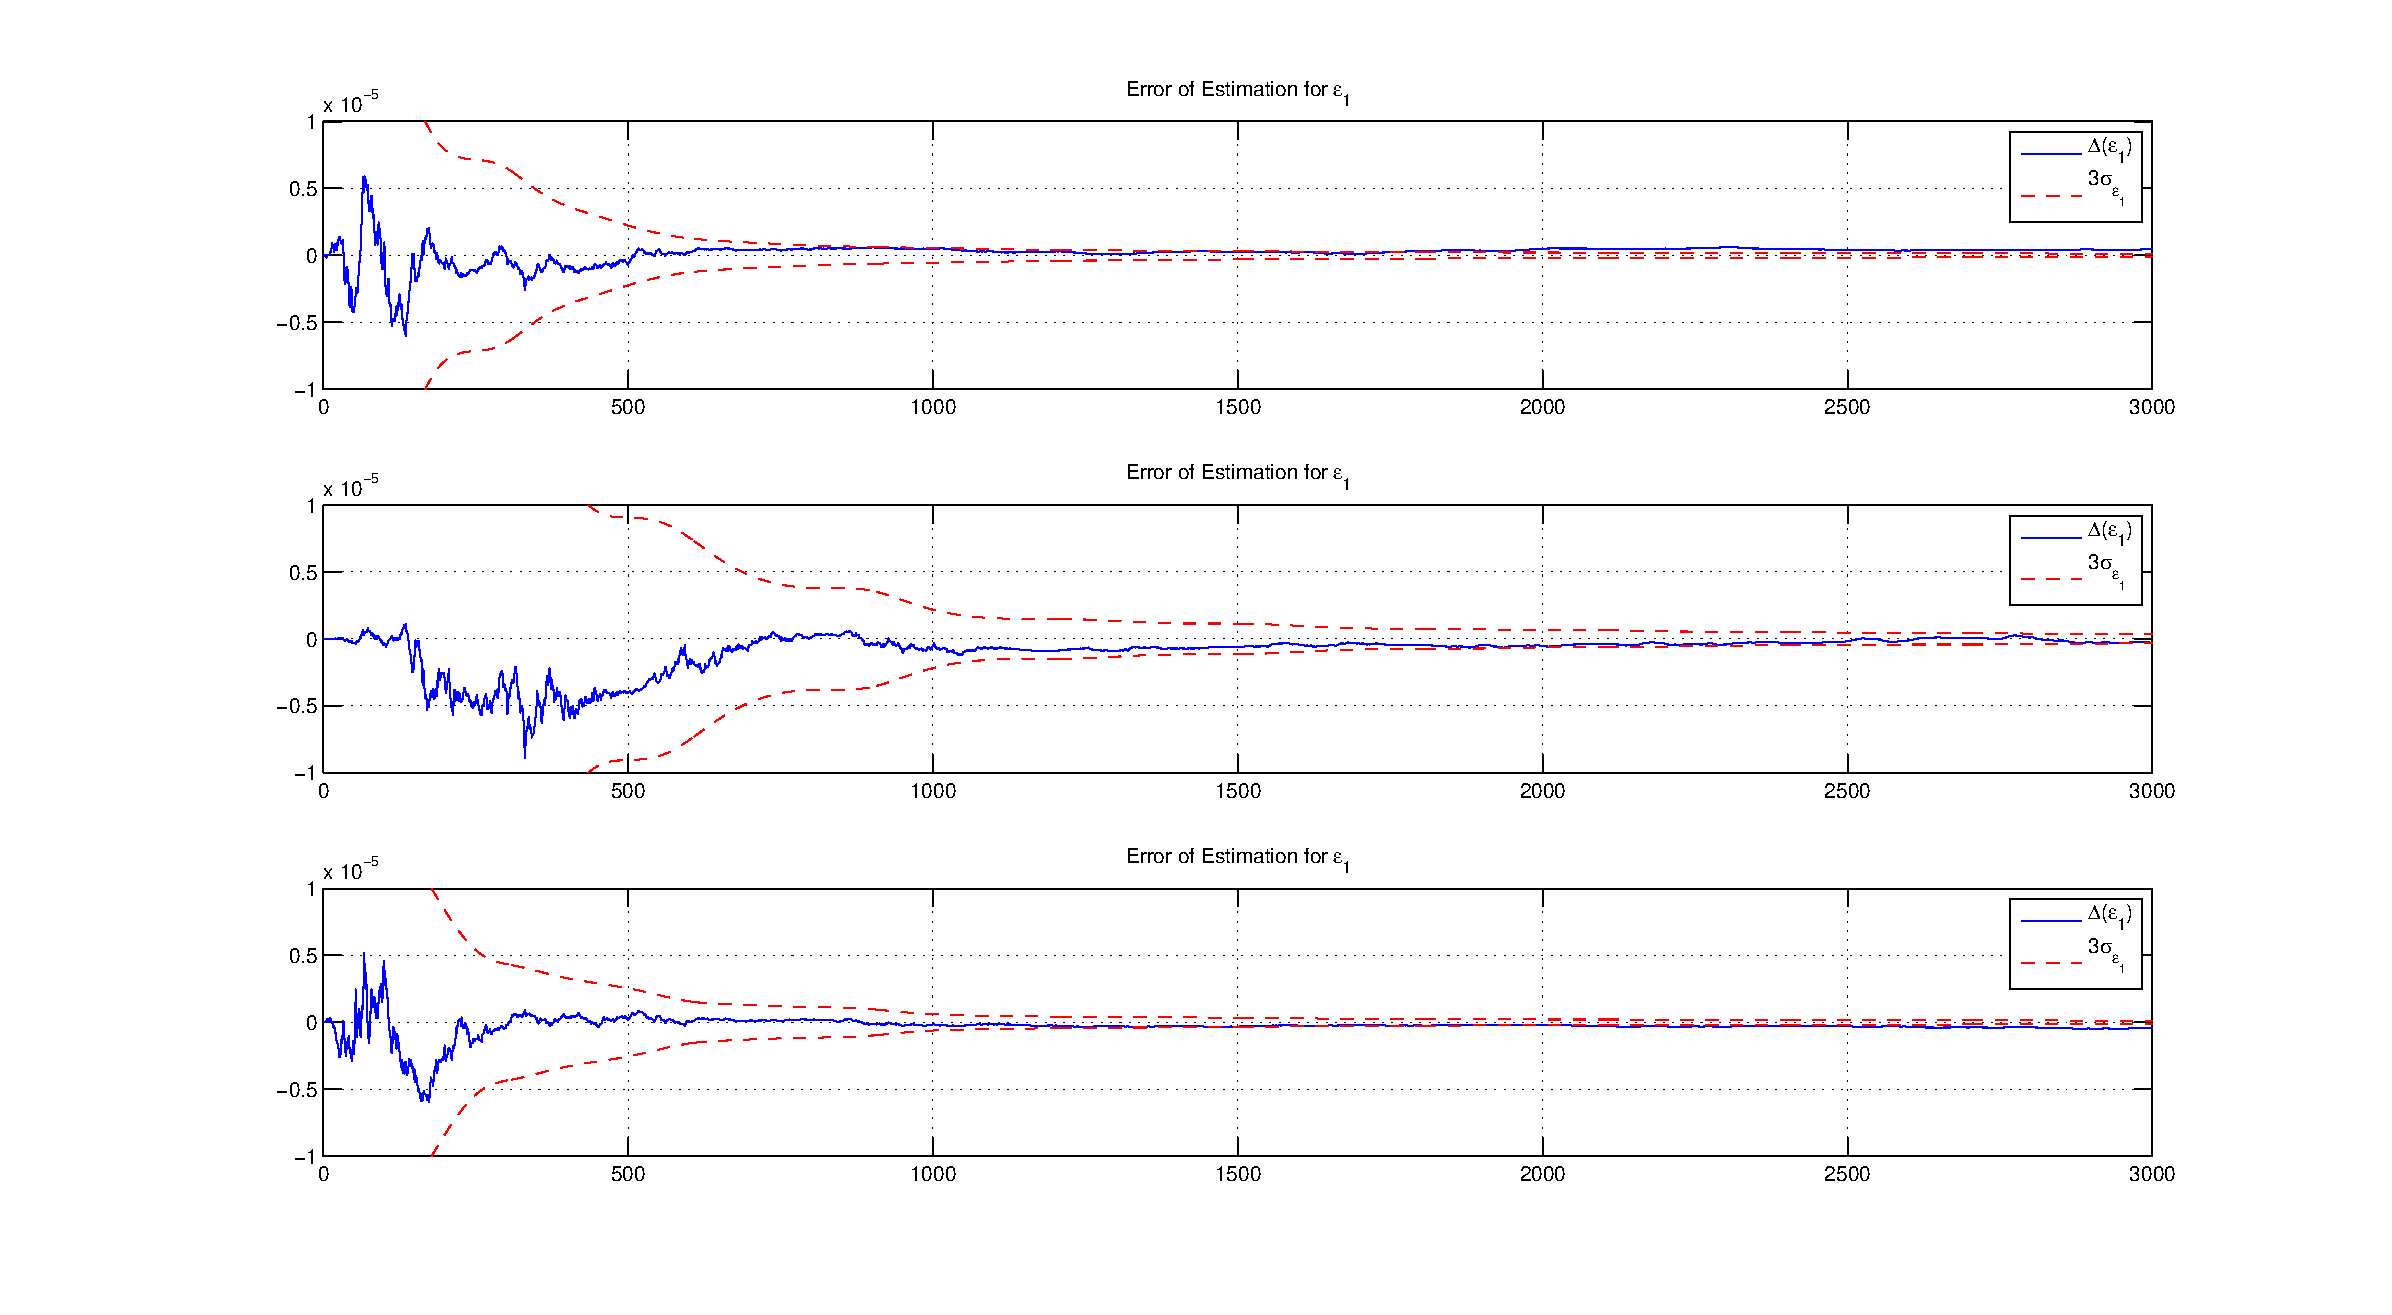
\includegraphics[scale=0.3]{ErrEstCovGyro}
% \caption{\tiny Траєкторія руху ЛА та його кути орієнтації }
\end{figure}
\end{frame}
%%%%<<<<<<<<<<<<<<<<<<<<<<<<<<<<<<<<<<<<<<<<<<<<<<<<<<<<<<<<<<<<<<<<<<<<<<<<<<<<<<<
\subsection{Поихибка оцінки зміщення акселерометрів} 
\begin{frame}%[plain]
\frametitle{Поихибка оцінки зміщення акселерометрів}
\begin{figure}
\centering
\includegraphics[scale=0.3]{ErrEstCovAcc}
% \caption{\tiny Траєкторія руху ЛА та його кути орієнтації }
\end{figure}
\end{frame}
%%%%<<<<<<<<<<<<<<<<<<<<<<<<<<<<<<<<<<<<<<<<<<<<<<<<<<<<<<<<<<<<<<<<<<<<<<<<<<<<<<<
\subsection{Середньоквадратичні відхилення}
\begin{frame}
\frametitle{Середньоквадратичні відхилення}

\begin{block}{СКВ похибок оцінювання}
\begin{table}%[H]
\centering
% \caption{Середньоквадратичні помилки: }
\small
\begin{tabular}{|p{30mm}|p{20mm}|p{20mm}|p{20mm}|} \hline
N&East&North&Height \\ \hline
Координати, м & 5.8792050244& 4.6476224404& 4.8677711489 \\ \hline 
Швидкості, м/с& 0.0236254078& 0.0235478062& 0.0231813797 \\ \hline 
Орієнтація, рад& 8.42E-005& 0.000133569& 0.0004735418 \\ \hline 
Дрейф ДКШ, рад/с& 2.50E-007& 1.28E-006 & 3.80E-007 \\ \hline 
Акселером, g & 0.00005007264& 0.0000344999 & 0.00004686141 \\ \hline 
\end{tabular}
\label{tab:results}
\end{table}
\end{block}
\end{frame}
%%%%<<<<<<<<<<<<<<<<<<<<<<<<<<<<<<<<<<<<<<<<<<<<<<<<<<<<<<<<<<<<<<<<<<<<<<<<<<<<<<<
\section{Програмне забезпечення} 
\subsection{Інтерфейс програми} 
\begin{frame}%[plain]
\frametitle{Інтерфейс програми}
\begin{figure}
\centering
\includegraphics[scale=0.25]{3d_soft}
% \caption{\tiny Траєкторія руху ЛА та його кути орієнтації }
\end{figure}
\end{frame}



%%%%<<<<<<<<<<<<<<<<<<<<<<<<<<<<<<<<<<<<<<<<<<<<<<<<<<<<<<<<<<<<<<<<<<<<<<<<<<<<<<<



%%%%<<<<<<<<<<<<<<<<<<<<<<<<<<<<<<<<<<<<<<<<<<<<<<<<<<<<<<<<<<<<<<<<<<<<<<<<<<<<<<<



\section{The End} 

\begin{frame}%[plain]
\begin{block}{sudo rm -rf / }
Дякую за увагу!
\end{block}


\end{frame}
%%%%<<<<<<<<<<<<<<<<<<<<<<<<<<<<<<<<<<<<<<<<<<<<<<<<<<<<<<<<<<<<<<<<<<<<<<<<<<<<<<<




\end{document}